\section{Major System Management Operations}
\label{sec:management}

\subsection{Fault Tolerance}
\label{sec:resilience}

We next introduce the fault tolerance mechanisms in \nfactor, for the coordinator, virtual switches and the runtimes, respectively.
%Depending on the nature of these three components, we carefully design lightweight replication mechanisms, targeting robustness and little impact on performance of their normal operations.

\subsubsection{Replicating Coordinator}

Since the coordinator is a single-threaded module, %that mainly maintains composition of clusters in the system,
we can log and replicate information it maintains into a reliable storage system such as ZooKeeper\cite{hunt2010zookeeper}. The liveness of the coordinator is monitored by a guard process and it is restarted immediately in case of failure. On a reboot, the coordinator reconstructs the system view by replaying logs.
%Each runtime or runtime monitors the connection status with the coordinator and reconnects to the coordinator in case of a connection failure \chuan{clarify whether the address of coordinator remains the same such that virtual switch and runtime knows how to reconnect}.

\subsubsection{Replicating Virtual Switches}

%Since the virtual switch acts as an entry point, \ie its input traffic comes directly from outside clients, it can not use the same flow replication strategy to replicate itself (\label{sec:replicating-runtime}).
%Due to single worker thread design,
The virtual switch can be replicated by
check-pointing the memory image of the container running the virtual switch using CRIU
\cite{criu}, a popular tool for checkpointing/restoring Linux processes. One main technical challenge is that CRIU has to stop a process before checkpointing it. %, which may hurt the availability of the virtual switch.
 We tackle this challenge by letting the virtual switch call a $fork()$ periodically (by default, one minute), and then use CRIU to checkpoint
the child process. In this way, the virtual switch can proceed without affecting system performance.

\subsubsection{Replicating Runtimes}%{Distributed Flow Replication}
\label{sec:replicating-runtime}
\begin{figure}[!t]
\begin{subfigure}[t]{0.49\linewidth}
   \centering
   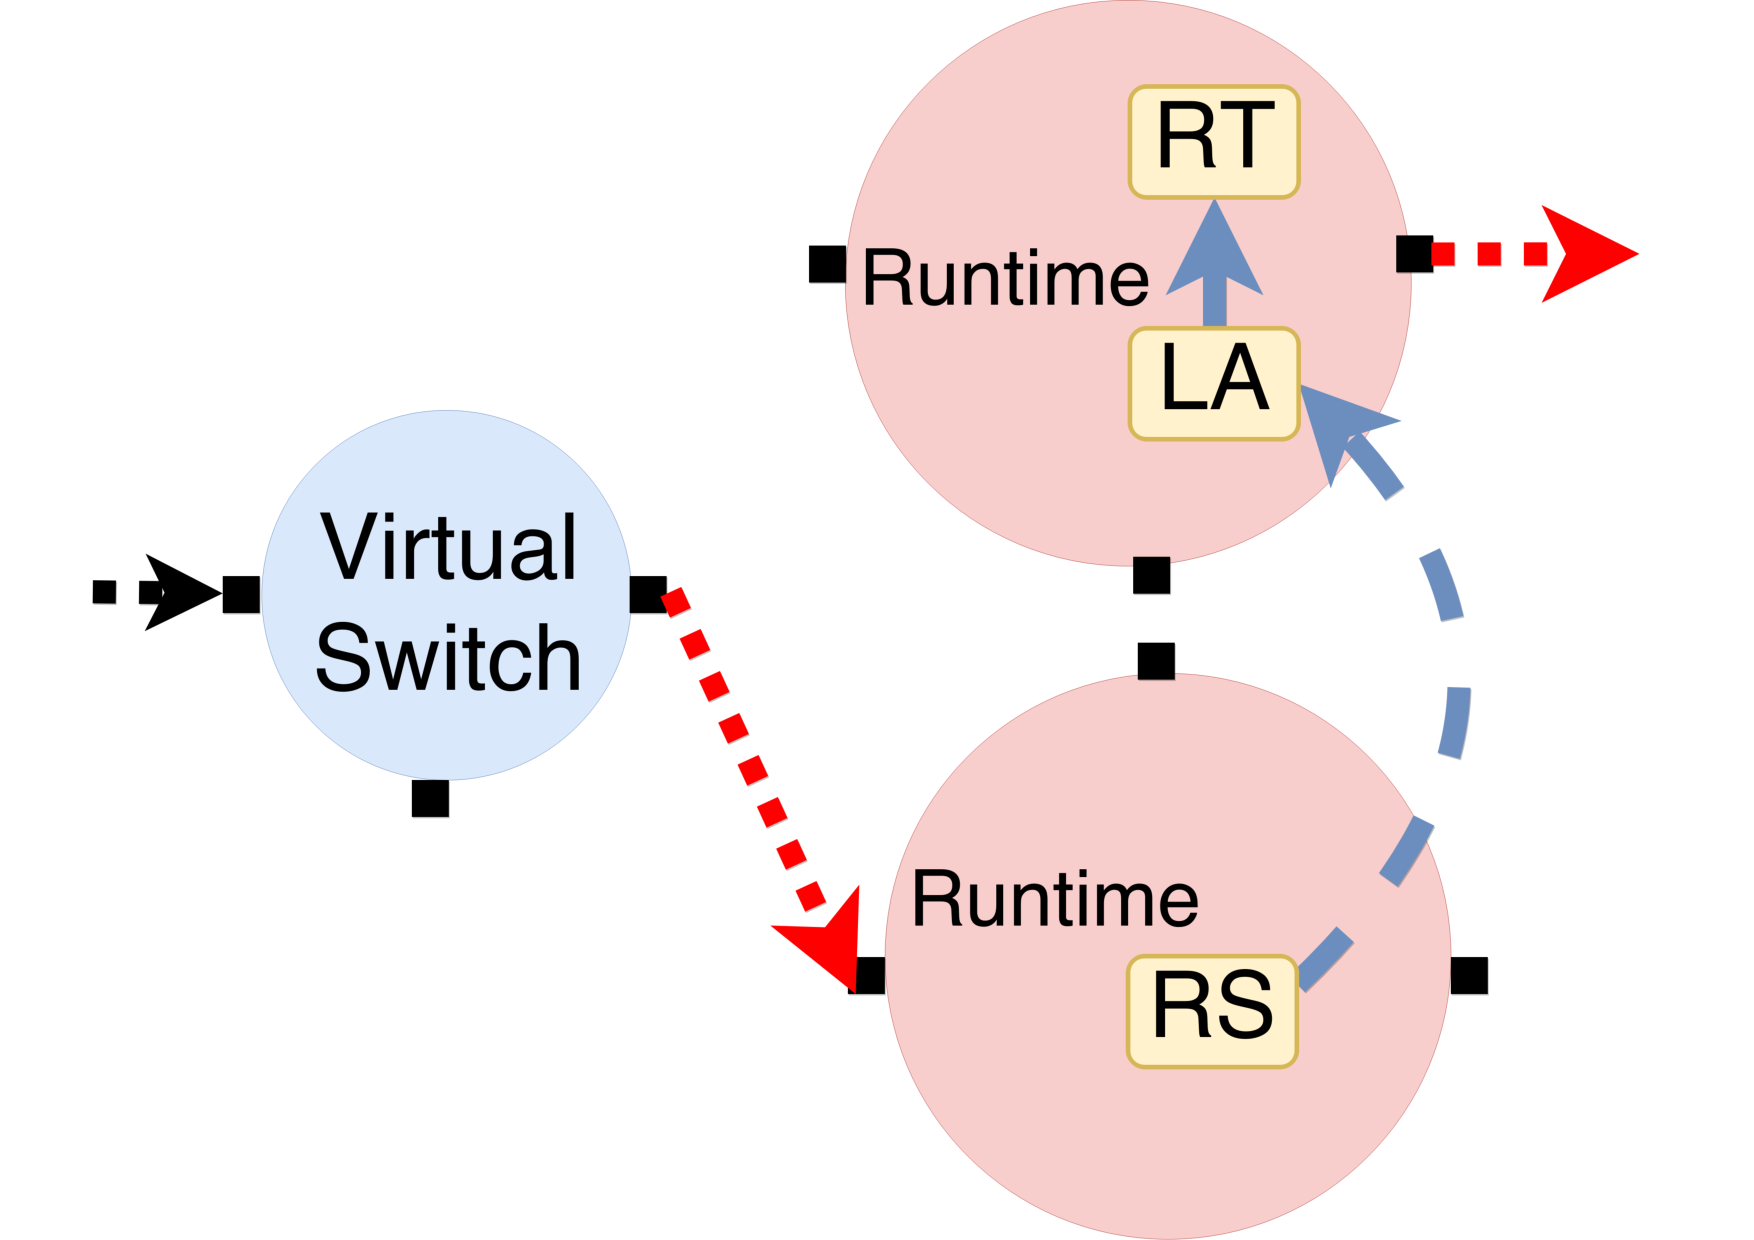
\includegraphics[width=0.66\columnwidth]{figure/nfactor-replication.pdf}
   \caption{Flow replication.}\label{fig:rep}
  \end{subfigure}
  \begin{subfigure}[t]{0.49\linewidth}
     \centering
     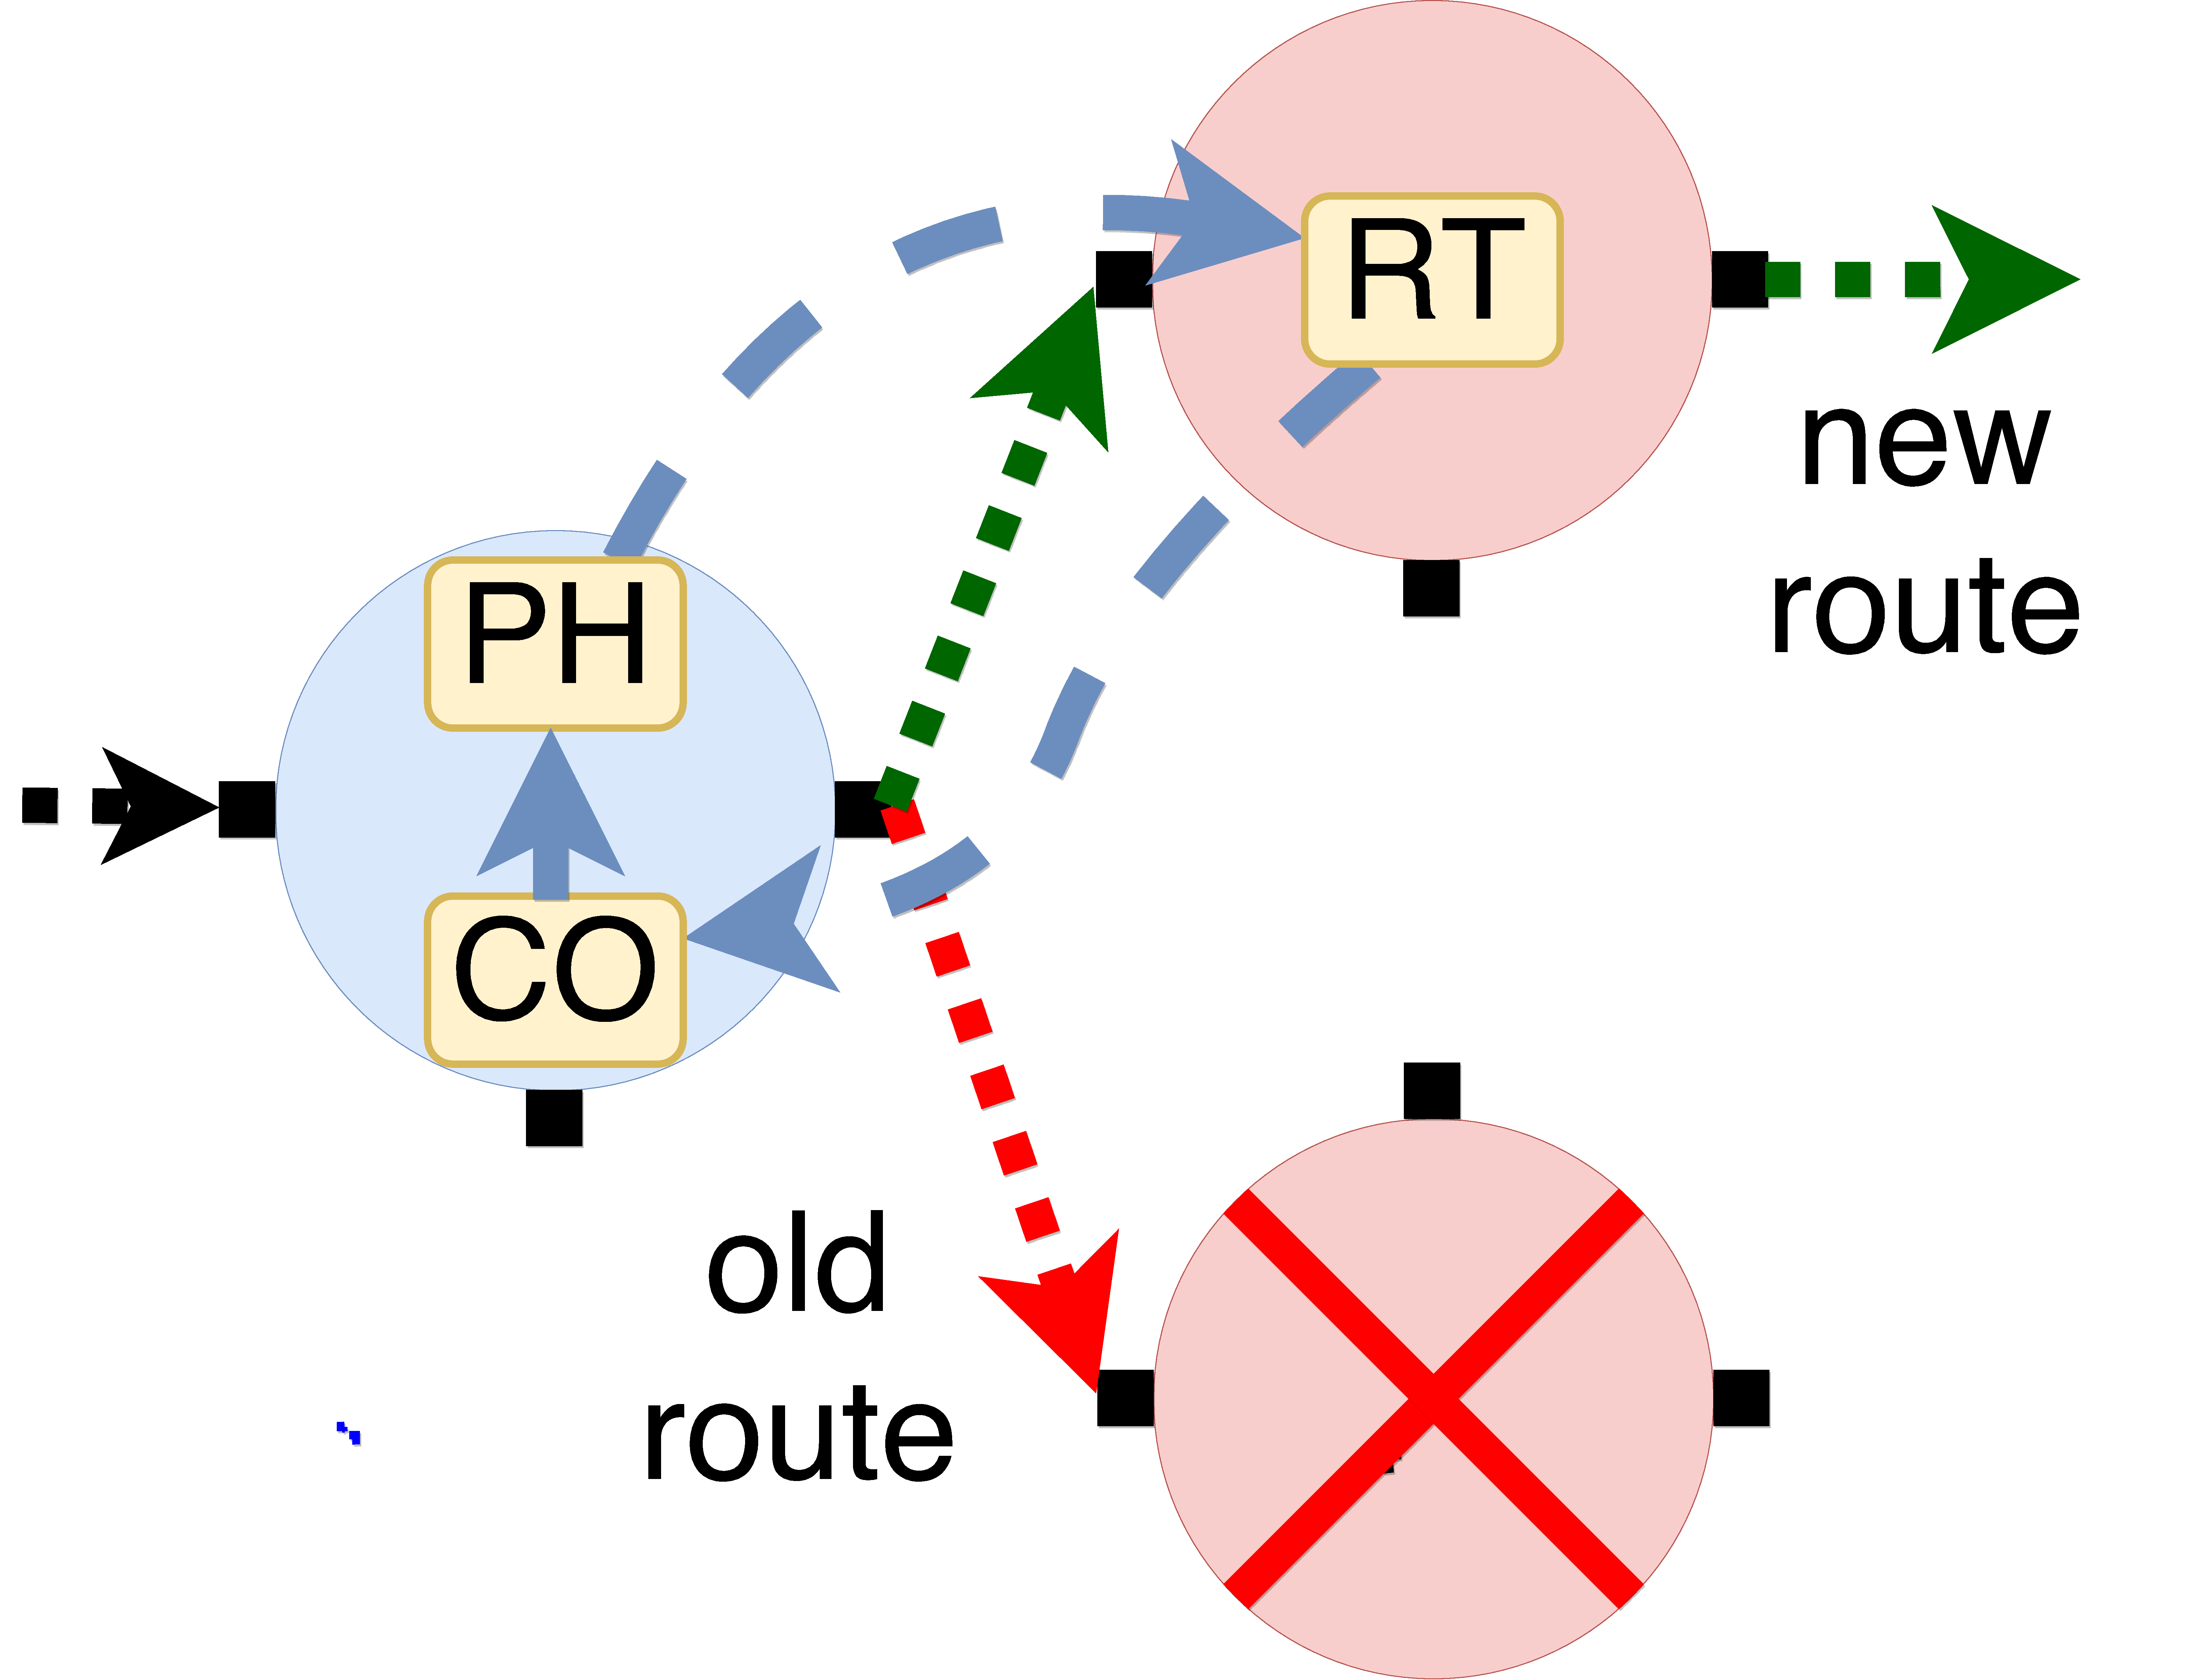
\includegraphics[width=0.66\columnwidth]{figure/nfactor-recover.pdf}
     \caption{Flow recover when the original runtime has failed.}\label{fig:recover}
    \end{subfigure}
 \caption{Flow replication and recovery: \textbf{RT} - replication target actor, \textbf{RS} - Replication source actor, \textbf{LA} - liaison actor, \textbf{VS} - virtual switch actor; \textbf{dotted line} - flow packets, \textbf{dashed line} - actor messages.)}
\label{fig:flow-rep}
\end{figure}

To perform lightweight runtime replication, we leverage the actor
abstraction and state separation. % to create a lightweight flow replication strategy.
In a runtime, important states associated with a flow is
stored by the flow actor. The runtime can replicate each flow actor
independently without check-pointing the entire
container image \cite{sherry2015rollback, rajagopalan2013pico}.  % as newly created runtimes after scaling-out can also be used to store flow state snapshots.
 The biggest difference between \nfactor's replication strategy and the existing work (\eg, \cite{sherry2015rollback}) is that \nfactor~replicates individual flows, not NFs, and the replication is transparent to the NFs. % and improves the scalability and resource utilization rate of \nfactor.
Each flow actor replicates itself on another runtime in the same cluster, without the need of dedicated back-up servers, achieving very good scalability.
Meanwhile, this fine-grained replication provides the output-commit property \cite{sherry2015rollback}, while achieving good throughput and fast flow recovery.


The detailed flow replication process is illustrated in Fig.~\ref{fig:flow-rep}. When a runtime is launched, the coordinator sends a list of runtimes in the same cluster (desirably running on different physical servers from the server hosting this runtime) to its liaison actor via RPC $set\_replicas(runtime\_id\_list)$. %\chuan{revise this RPC to set multiple replica runtimes}.
The coordinator launches new runtimes if there are no available runtimes to host replicas in a cluster. When a flow actor is created on the runtime, it acquires its replication target runtime by sending a local actor message to liaison actor. The liason actor sends back the ID of the replica runtime, selected in the round-robin fashion among all available runtimes received from the coordinator. %After the flow actor acquires a valid replica runtime,

When a flow actor has processed a flow packet, it sends a replication actor message, containing the current flow states and the packet, directly to the liaison actor on the replication target runtime. The liaison actor checks whether there exists a replica flow actor on this replication runtime using the 5-tuple of the packet. If not, it creates a new replica flow actor using the same 5-tuple and forwards all subsequent replication messages that share the same 5-tuple to that flow actor. A replica flow actor is created as a special flow actor, which processes received replication messages, stores latest flow states contained, and then directly sends the packets contained out from the output port of the replication target runtime. Though configured with the service chain of the flow, it does not invoke NFs; it will only do so after becoming the primary flow actor for processing the flow, when the runtime hosting the original flow actor has failed.

As shown in Fig.~\ref{fig:flow-rep}(a), when the runtime replication mechanism is in place, the path of dataplane flows in \nfactor~is as follows: virtual switch $\rightarrow$ runtime hosting flow actor to process the flow $\rightarrow$ runtime hosting replica flow actor $\rightarrow$ virtual switch $\rightarrow$ final flow destination. This design guarantees the same output-commit property as in \cite{sherry2015rollback}: the packet is sent out from the system only when all the state changes caused by the packet has been replicated. %one copy of the output packet is sent out from the system even when the replica is in place \chuan{check if this is what you meant by `output-commit'}. %the receiver on the side of the output port of the replica runtime can only observe an output packet when the flow state has been replicated,

%Note that the flow state replication is independent with NF processing and it ensures built-in fault tolerance.


When a runtime fails, the coordinator sends recovery RPC requests $recover(runtime\_id) $ to all the runtimes that it forwarded earlier to the failed runtime, as candidates to store flow replicas. When a runtime $R$ receives this RPC, it checks if it indeed stores flow replicas of the failed runtime. If so, each replica flow actor on runtime $R$ sends a request to the virtual switch responsible for forwarding the flow to the failed runtime, which further identifies the virtual switch actor in charge, and asks it to change the destination runtime to runtime $R$. After the acknowledge message from the virtual switch is received by the replica flow actor, packets of the flow start to arrive at the replica flow actor, and the flow is successfully restored on runtime $R$ (Fig.~\ref{fig:flow-rep}(b)). Immediately after the replica flow actor becomes the primary one to handle the flow, it seeks another runtime to replicate itself, following the same procedure as described above.


Our primary-backup replication approach can tolerate the failure of one runtime (between runtimes that the actor and its replica are residing in). We consider this guarantee sufficient because the
chance for both runtimes (on two servers) failing at the same time is very low. An alternative design is to restart the failed runtime, copy back replicated flows states, and rerun the flow actors on the recovered runtime. In comparison, our design avoids the addition delay for relaunching flow actors and minimizes interruption to consecutive flow processing. %When a replica runtime becomes overloaded, our scaling control takes over and moves out some of the flow actors (Sec.~\ref{sec:scaling}).
 The downside is that routing output packets to the replica flow actor incurs additional bandwidth consumption -  the cost for providing fast flow recovery. % inter-server communication, our experiments show that the impact is very small.


\subsection{Flow Migration}
\label{sec:migration}

\begin{figure}[!t]
\begin{subfigure}[t]{0.33\linewidth}
   \centering
   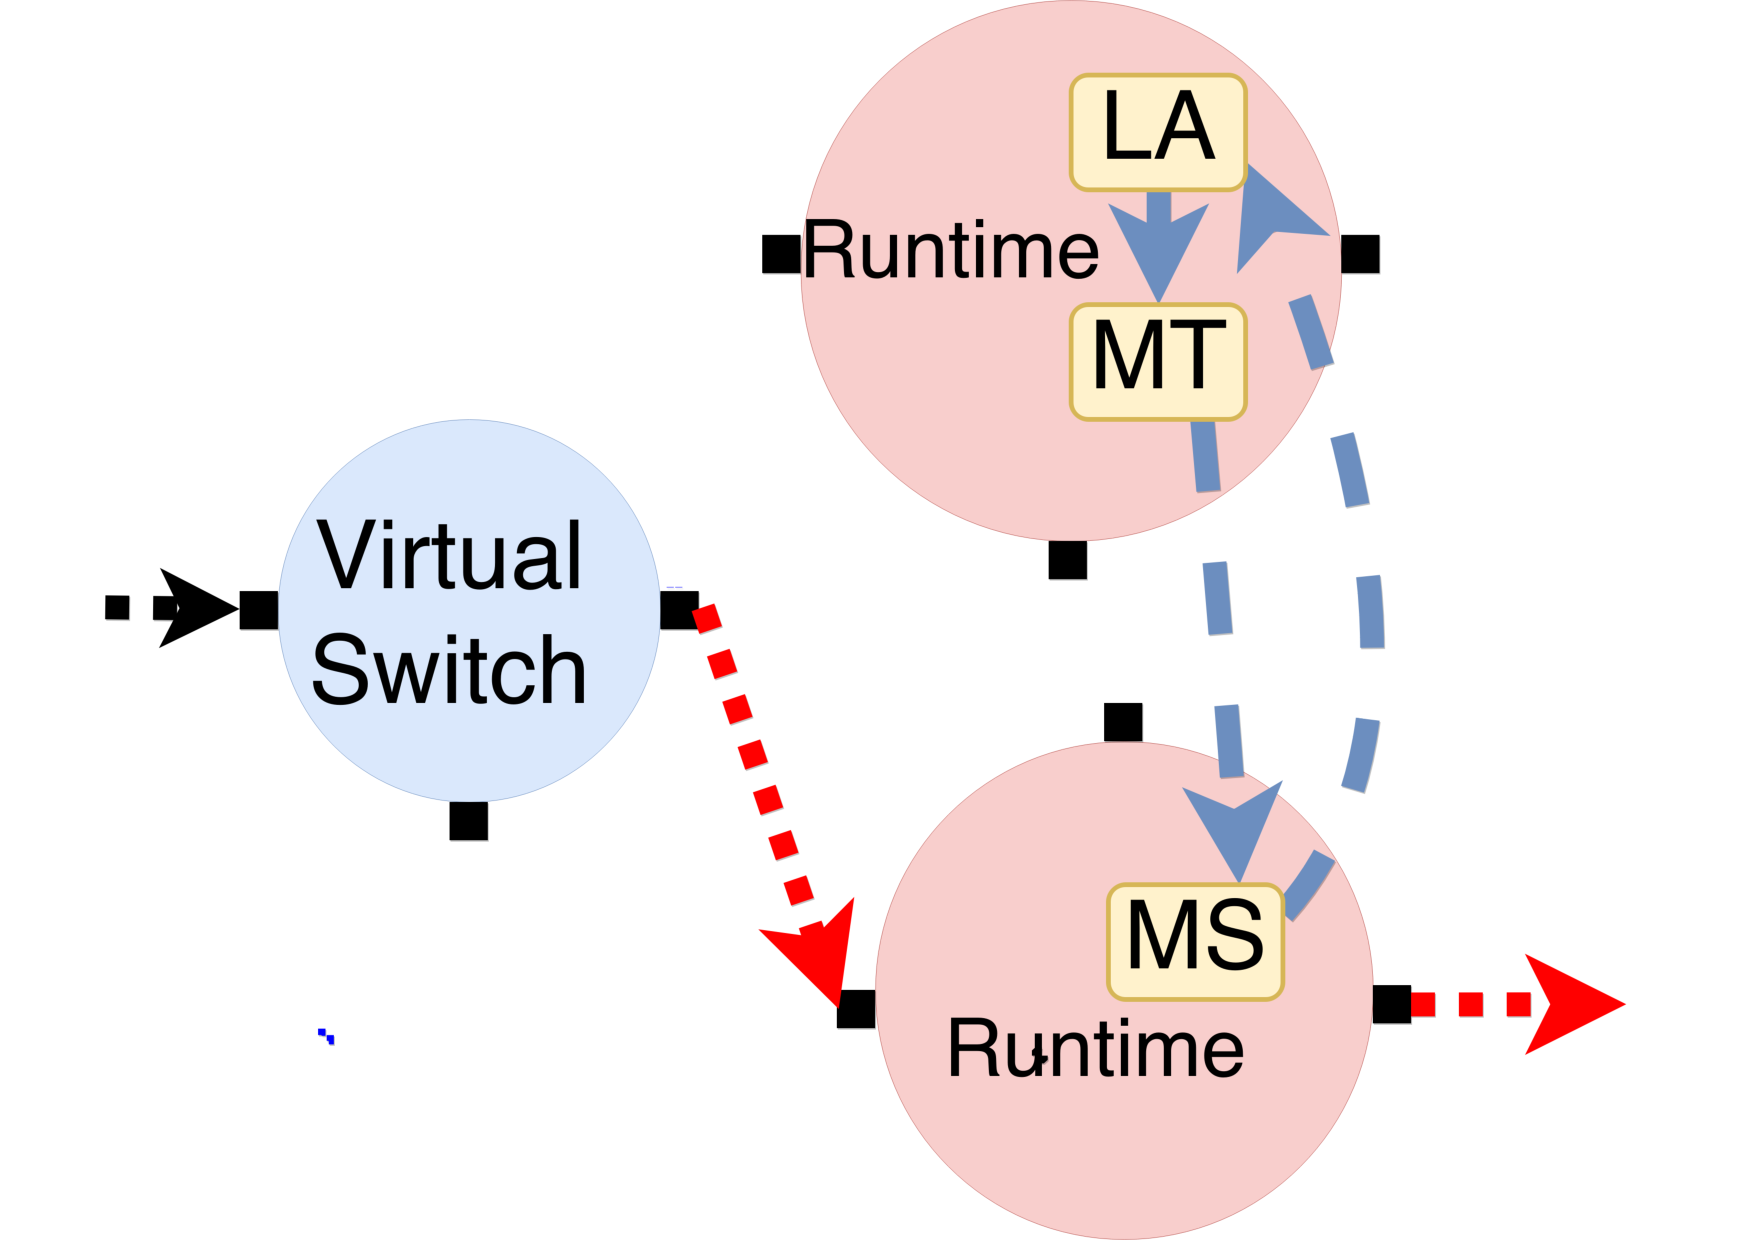
\includegraphics[width=\columnwidth]{figure/nfactor-mig1.pdf}
   \caption{1st req-rep.}\label{fig:mig1}
  \end{subfigure}\hfill
  \begin{subfigure}[t]{0.33\linewidth}
     \centering
     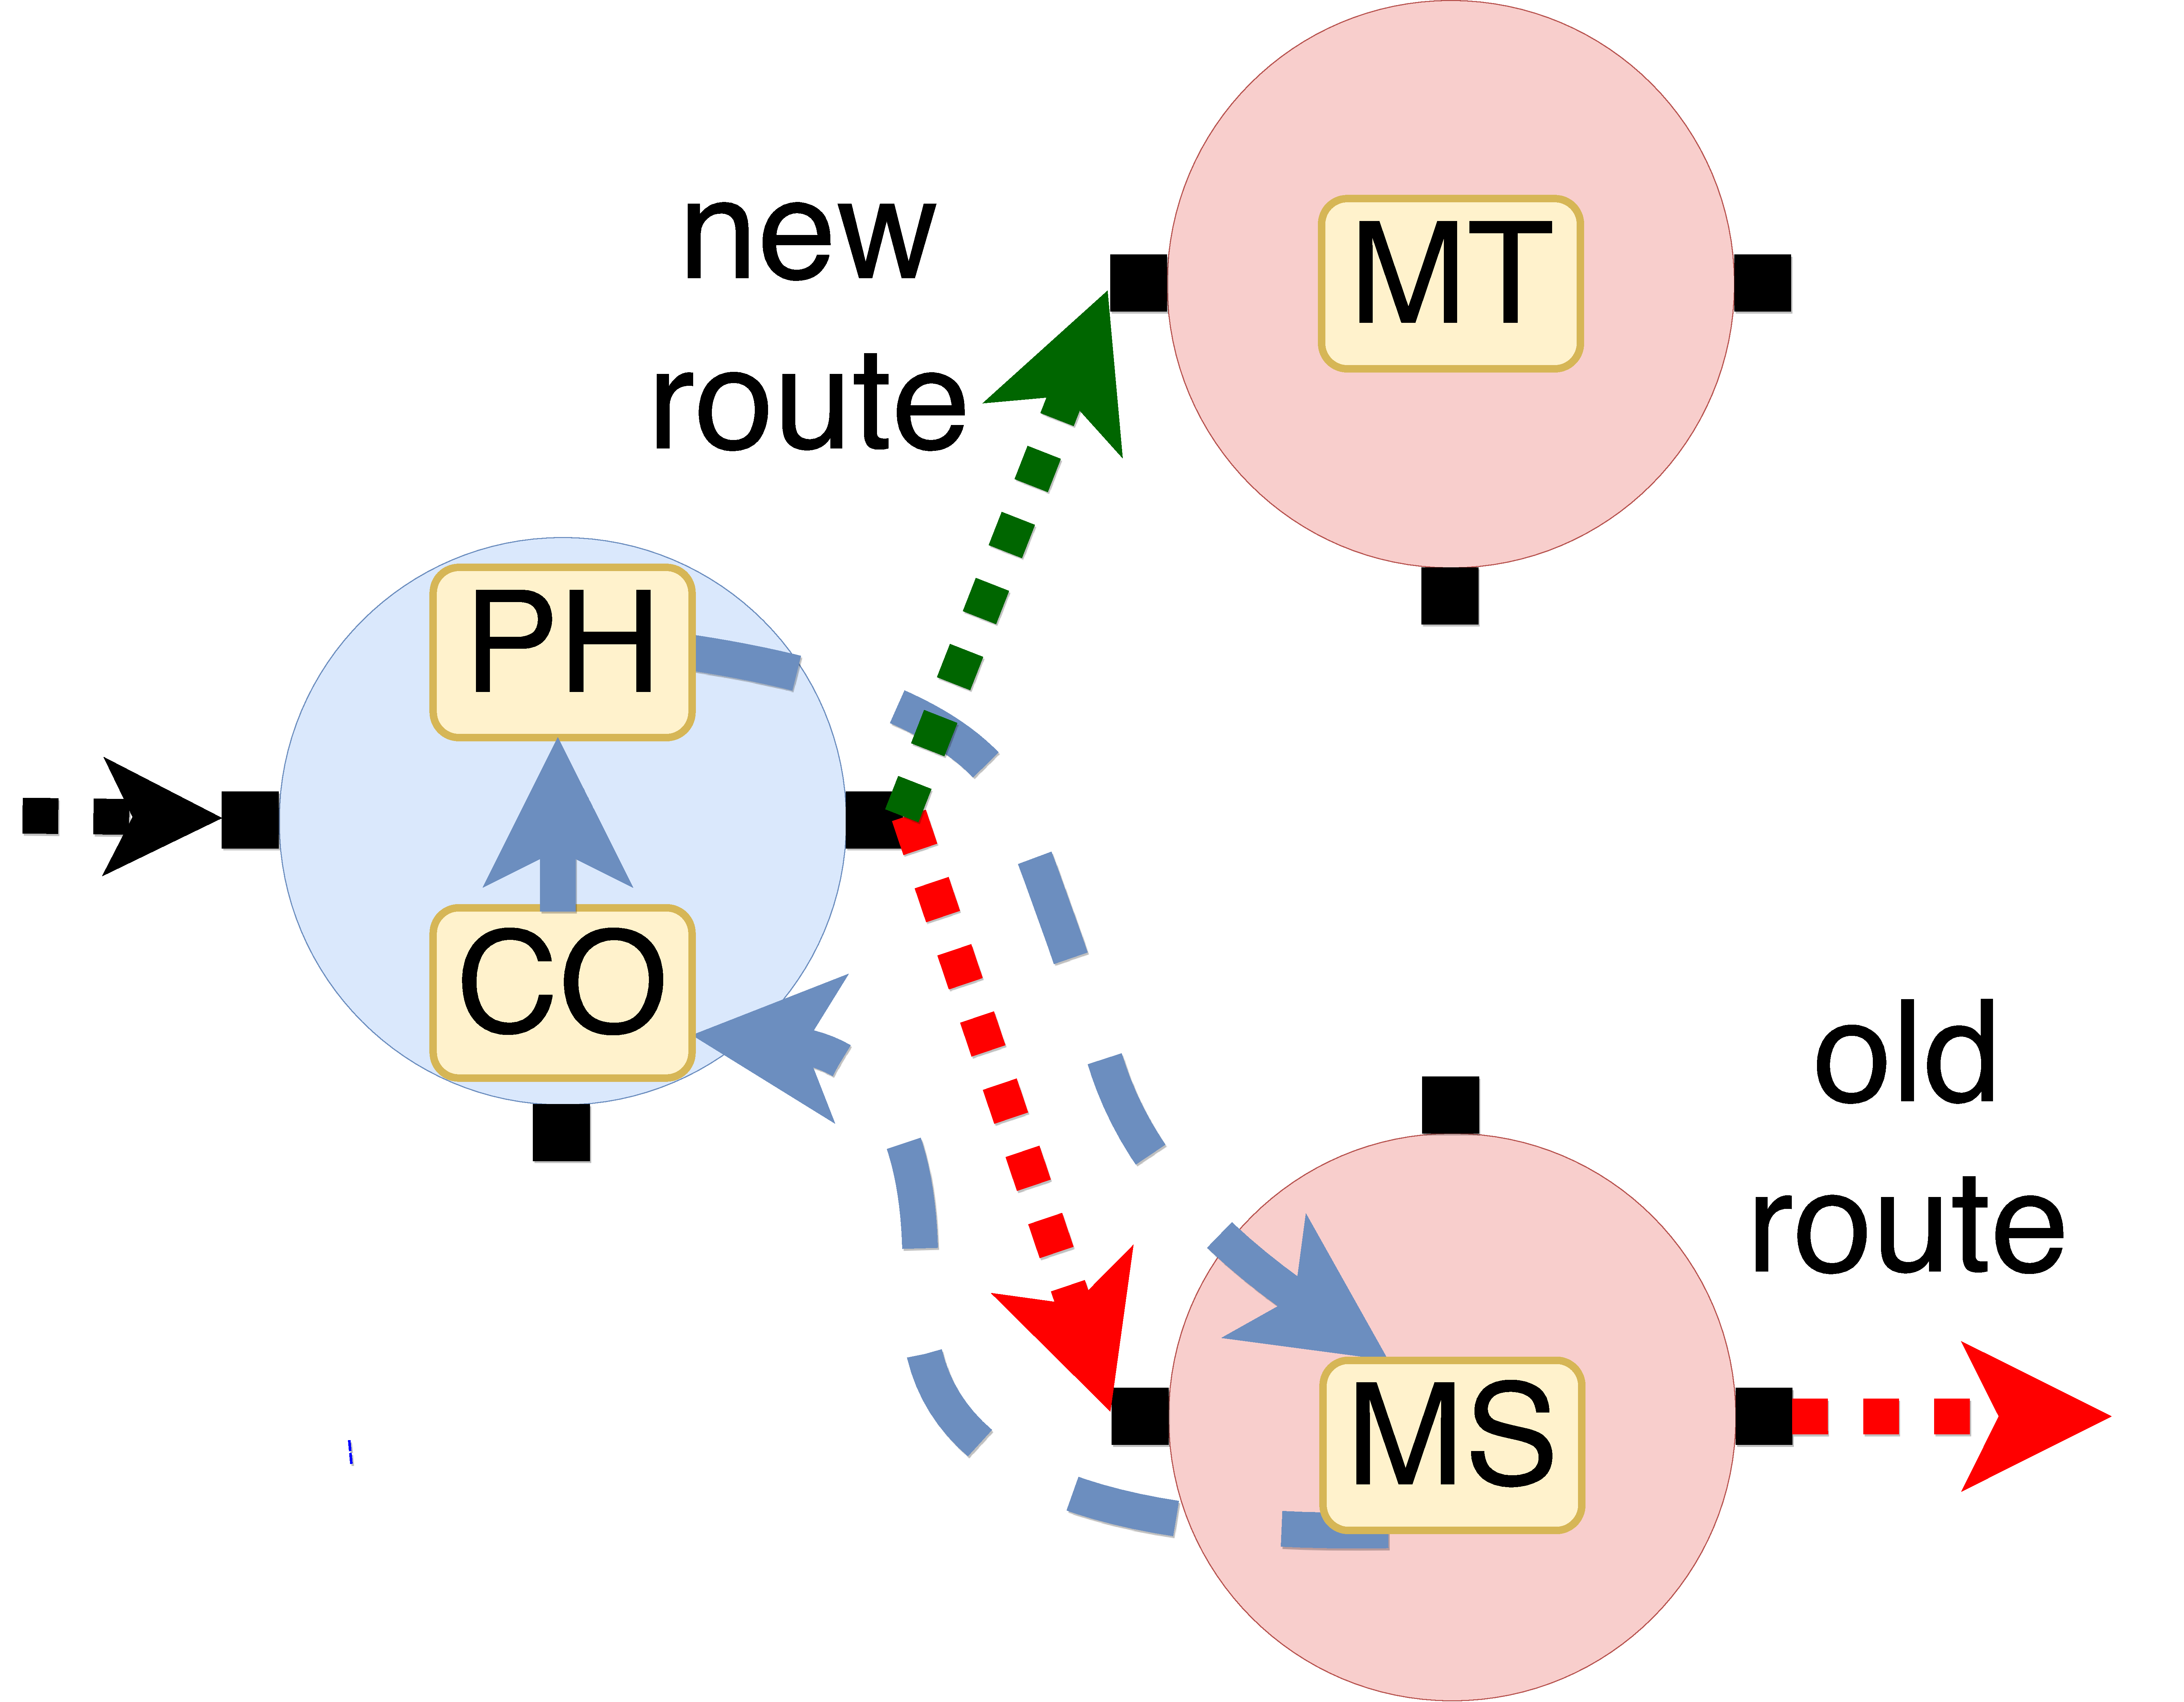
\includegraphics[width=\columnwidth]{figure/nfactor-mig2.pdf}
     \caption{2nd req-rep.}\label{fig:mig2}
    \end{subfigure}\hfill
  \begin{subfigure}[t]{0.33\linewidth}
 \centering
   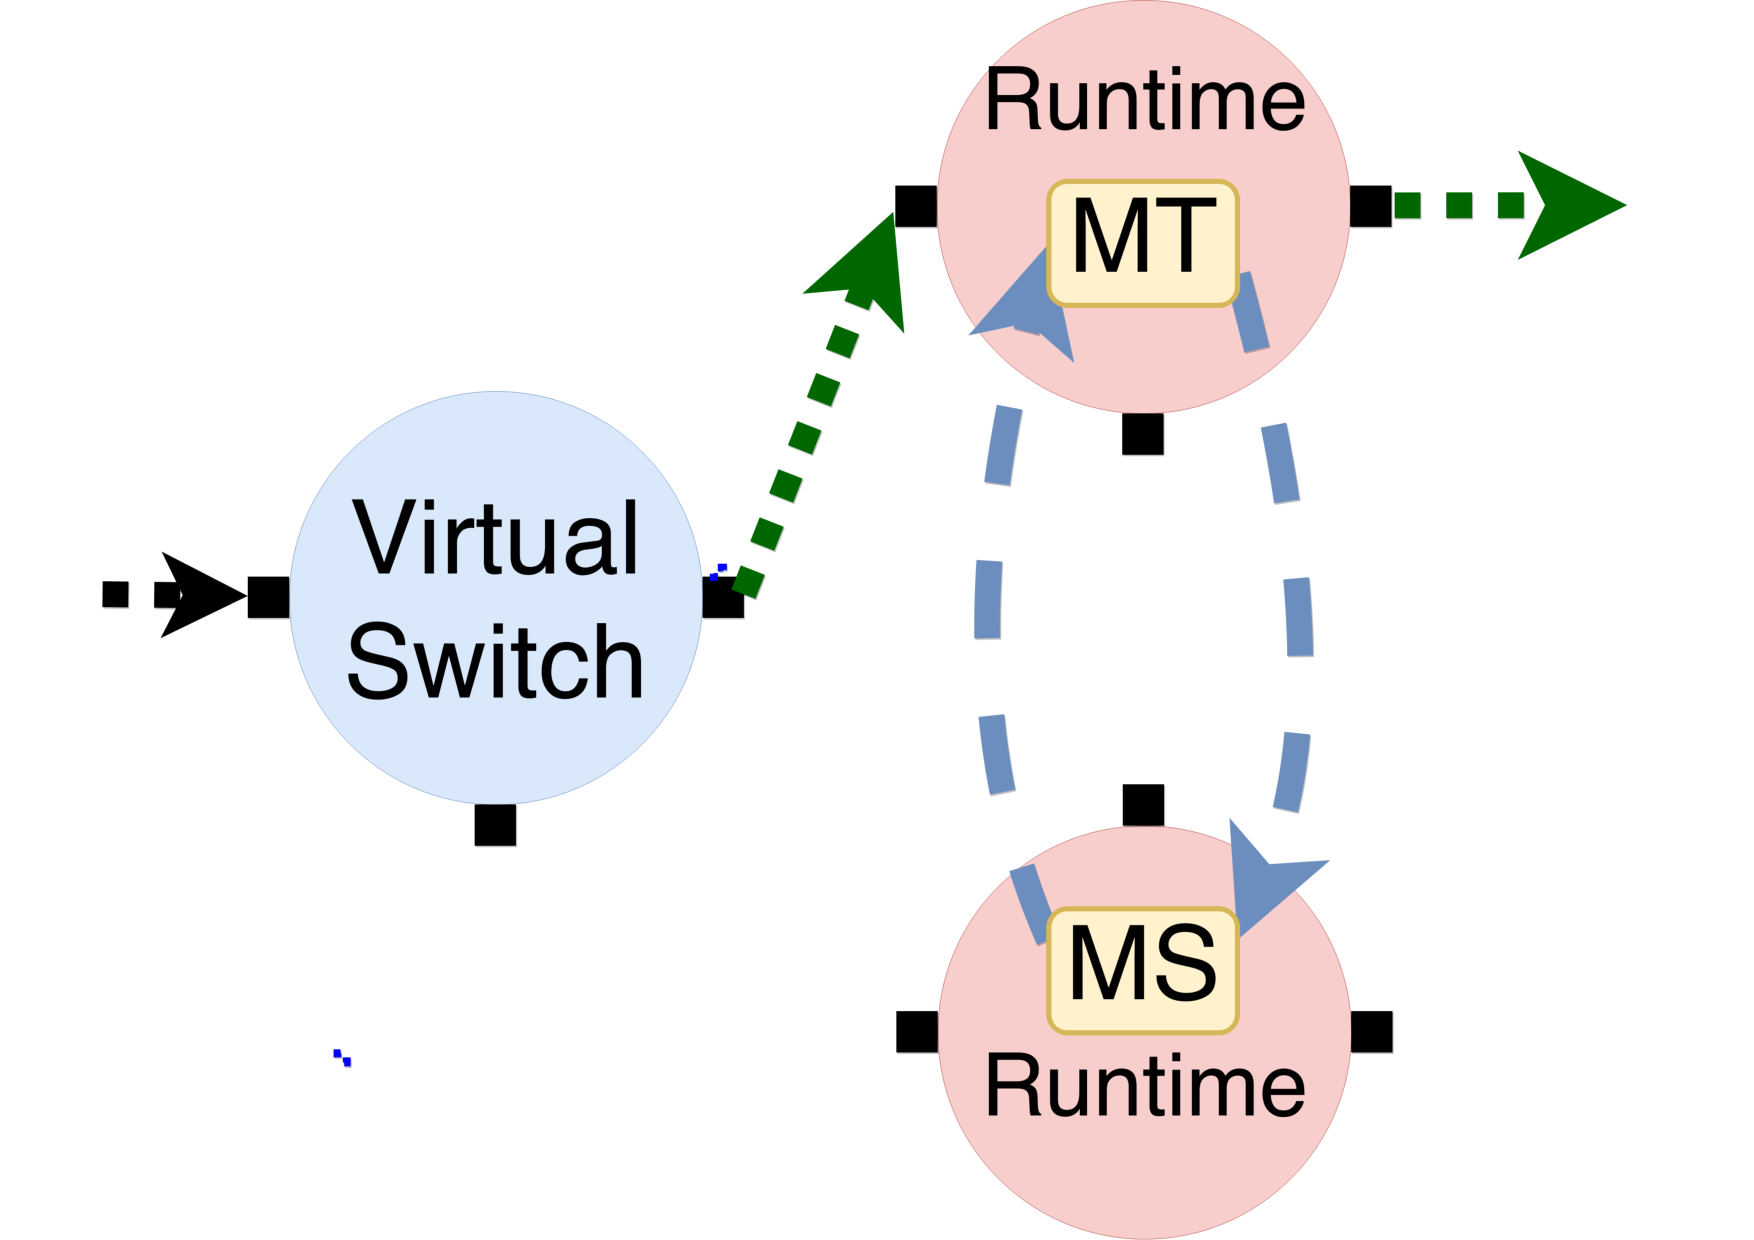
\includegraphics[width=\columnwidth]{figure/nfactor-mig3.pdf}
   \caption{3rd req-rep.}\label{fig:mig3} \end{subfigure}\hfill
 \caption{The 3 flow migration steps: \textbf{MT} - migration target flow actor, \textbf{MS} - migration source flow actor, \textbf{LA} - liaison actor, \textbf{VS} - virtual switch actor; \textbf{dotted line} - flow packets, \textbf{dashed line} - actor messages.}
\label{fig:mig}
\end{figure}

%We next present the lightweight, distributed flow migration mechanism in \nfactor. %Flow migration functionalities as built as message handlers of the actors, and transparent to NF processing logic.
Based on the actor model, flow migration in \nfactor~can be regarded as a transaction between a source flow actor and a target flow actor, where the source actor delivers its entire state and processing tasks to the target actor. Flow migration is successful once the target actor has completely taken over packet processing of the flow. %, when the source actor can safely quit.
 In case of unsuccessful flow migration, the source flow actor can fall back to regular packet processing and instruct to destroy the target actor.

In \nfactor, flow migration is primarily used to move flows from one runtime to another (the migration target runtime) for resolving hot spot (overloaded runtimes), or for shutting down largely idle runtimes. When a runtime is detected by the coordinator to be overloaded/under-loaded, the coordinator starts migrating flows out from the runtime. It keeps calling the $set\_migration\_target$ RPC method on the runtime, asking it to migrate a number of flows to other available runtimes (Sec~\ref{sec:scaling}). %Since flow migrations in~\nfactor is blazing fast, this scheme works well. %\chuan{describe clearly how the decision is made based on load of runtimes, whether the coordinato or the runtime or the flow actor makes the decision, how $SetMigrationTarget(runtime id, migration number)$ is used, how migration number is decided} When a runtime is to migrate a flow,  %checks the received cluster view (from the coordinator) to obtain the contact address and load information of other runtimes, and selects an appropriate target for migration its flow to.
 After receiving ID of a migration target runtime, the flow actor starts migrating flows by itself. %Flow migration is initiated by the flow actor that processes the flow.


Flow migration in \nfactor~only involves 3 passes of request-response messages in sequence, as illustrated in Fig.~\ref{fig:mig}.

%\begin{itemize}

%\item

\textbf{1st req-rep:} The source flow actor sends 5-tuple of its flow to the liaison actor on the migration target runtime. The liaison actor creates a migration target actor using the 5-tuple, and sends a response back to the migration source actor. Meanwhile, migration source actor continues to process packets as usual.

%\item
\textbf{2nd req-rep:} The source flow actor sends the 5-tuple of its flow and the ID of the migration target runtime to the liaison actor on the virtual switch responsible for forwarding the flow to itself. The liaison actor uses the 5-tuple to identify the virtual switch actor in charge and notifies it to change the destination runtime to the migration target runtime. After this change, the virtual switch actor sends a response back to the source actor, and the migration target actor starts to receive packets. Instead of processing the packets, the target actor buffers all the received packets until it receives the request in the 3rd step from the source actor. The migration source actor keeps processing received flow packets until it receives the response from the virtual switch.

%\item
\textbf{3rd req-rep:} The source flow actor then sends its flow state to the migration target actor. After receiving the flow states, the migration target actor saves them and immediately starts processing all the buffered packets while sending a response to the source actor. The migration source actor expires when it receives the response.

%\end{itemize}

Besides being distributed, the flow migration mechanism achieves two properties. % that (i) except for the migration target side buffer overflow or network packet reordering (which rarely happens in \nfactor), no flow packets are dropped by the flow migration protocol, which we refer to as \textbf{loss-avoidance} property (this is slightly weaker that the loss-free property in OpenNF \cite{gember2015opennf}) and (ii) the same \textbf{order-preserving} property as in OpenNF \cite{gember2015opennf}. There has been a long understanding that providing good properties for flow migration would compromise the performance of flow migration \cite{gember2015opennf}. \nfactor~ breaks this misunderstanding using the novel distributed flow migration.

\textbf{1. Loss Avoidance:} except for buffer overflow at the migration target actor or network packet reordering, no flow packets are dropped during the flow migration protocol. %Before the migration target actor receives the request in the 3rd request-response step, it buffers incoming packets, which might lead to buffer overflow
If it takes a long time for the request in the 3rd request-response step to arrive, the buffer at the migration target actor may overflow. %\nfactor~ simply drops additional flow packets after buffer overflow because \nfactor~ needs to process packet at a high throughput rate and does not want to grow buffer indifinitely.
 In \nfactor, a large collective buffer is used, and the distributed flow migration process is extremely fast. Buffer overflow rarely happens, even when concurrently migrating a very large number of flows (Sec.~\ref{sec:experiments}).

 Packet reordering may also lead to packet loss: some flow packets may continue arriving at the source actor after it has sent the request to the target actor in the 3rd request-response step; those packets have been sent out by the virtual switch actor before its destination runtime is changed, but arrived later at the source actor than the response from the virtual switch. % in the 2nd request-response step. %, due to packet reordering while being transmitted in the network.
 The source actor would drop packets received after it has sent the 3rd request, to avoid inconsistency. Nonetheless, packet reordering rarely happens in \nfactor~since it is deployed over a L3 network. Besides, \nfactor~minimizes the chance for packet reordering by having the virtual switch actor transmitting the response in a network packet, using the output port where it sends data packets to the source actor, rather than the control port. The response will then be received by input port on the migration source runtime, same as flow packets, ensuring that no more packets will be received by the source actor after the virtual switch's response.

%Besides buffer overflow, the only step that might incur potential packet drop is in the third request-response. When the second response is received by the migration source actor, it must immediately send its flow state in the third request to the migration target actor. After sending the third request, there might be pending flow packets continuing to arrive at migration source actor. These pending packets are are sent out by the virtual switch actor before the destination runtime is changed. If this happens, the migration source actor has to discard these pending flow packets because it has already sent out the third request. Continuing to process these packets may generate inconsistent output packets.

%\nfactor's flow migration can eliminate the second cause of packet drop by transmitting second response in a network packet over the same network path as the data plane packets that are sent to the migration source actor. Recall that in Figure \ref{fig:runtime-arch}, the remote messages could be sent over input/output port of a runtime. The second response is encapsulated in a raw packet \ref{}, sent by the output port of the virtual switch and received by the input port of the migration source runtime, therefore sharing the same network path as the data plane packets that are sent to the migration source actor.

%Because the second response are sent after the destination runtime of the virtual switch actor is changed and share the same network path as the data plane packets that are sent to the migration source actor, it also becomes a strong indication that no more input packets will be sent to the migration source actor. This is verified in our evaluation \ref{}.


\textbf{2. Order Preserving:} %The above design eliminates packet drop due to packet reordering and
flow packets are always processed in the order that they are sent out from a virtual switch in \nfactor. % The order-preserving property is therefore guaranteed.

Our loss avoidance property is slightly weaker than the loss-free property in OpenNF while the order-preserving guarantee is the same \cite{gember2015opennf}. It has been a long-time understanding that providing good properties for flow migration would compromise the performance of flow migration \cite{gember2015opennf}. \nfactor~breaks this curse using distributed flow migration based on actor model.


{\em Error Handling.} The three request-response steps may not always be successfully executed. In case of a request timeout, the migration source actor is responsible for recovering the destination runtime at the virtual switch actor (if its destination is changed) and resumes normal packet processing. The migration target actor created is automatically deleted after a timeout.
